\documentclass[10pt,aspectratio=1610]{beamer} % use option aspectratio=169 or 1610 for wide slides
% Note: For online presentations via Zoom use the ratio of the screen you want to share
\usetheme{Rochester}

% load syscop style
\usepackage{style/syscop}

%--------------------------------------------------
% TITLE
%--------------------------------------------------

% NOTE: what's in [ ] goes to footer for the fields title, author and date
\title[Short Report on Riccati Solver]{\huge Short Report on Riccati Solver}


%--------------------------------------------------
% Useful packages
%--------------------------------------------------

\usepackage{mathtools}
\usepackage{mathdots}
\usepackage{graphicx}
\usepackage{optidef}
\usepackage{booktabs}
\usepackage{diagbox}
\usepackage{multirow}
\usepackage{geometry}
\usepackage{subcaption}
\usepackage{nicematrix}

\begin{document}

\InsertTitle

\begin{frame}
    \frametitle{Quick update}
    Several quick updates on my current progress:
    \begin{itemize}
        \item Highly similar (or nearly identical) prototype solver to the HPIPM on convex QPs is implemented
        \item A heuristic modification on algorithm: Mehrotra predictor-corrector to Mehrotra probing for nonconvex QPs.
        \item Some preliminary proof for local quadratic convergence rate on current algorithm is attempted
        \item A globalization strategy, funnel line search, is implemented in prototype solver, but proof is not attempted yet.
    \end{itemize}
\end{frame}

% Ensure \usepackage{amsmath} is included in your document preamble
\begin{frame}
    \frametitle{Prototype update}
    The prototype solver is implemented to solve the following QP:
    \begin{equation*}
    \begin{aligned}
        & \underset{x, u}{\text{minimize}} 
        & & \sum_{k=0}^{N-1} \frac{1}{2} \begin{bmatrix} x_k \\ u_k \end{bmatrix}^T \begin{bmatrix} Q_k & S_k^T \\ S_k & R_k \end{bmatrix} \begin{bmatrix} x_k \\ u_k \end{bmatrix} + \begin{bmatrix} q_k \\ r_k \end{bmatrix}^T \begin{bmatrix} x_k \\ u_k \end{bmatrix} + \frac{1}{2} x_N^T Q_N x_N + q_N^T x_N \\
        & \text{subject to} 
        & & \begin{aligned}[t]
                & \quad x_0 = \bar{x}_0, \\
                & \quad x_{k+1} = A_k x_k + B_k u_k, \quad k = 0, \dots, N-1, \\
                & \quad \begin{bmatrix} \underline{u}_k \\ \underline{x}_k \\ \underline{d}_k \end{bmatrix} \le \begin{bmatrix} J_k^{b,u} & 0 \\ 0 & J_k^{b,x} \\ D_k & C_k \end{bmatrix} \begin{bmatrix} u_k \\ x_k \end{bmatrix} \le \begin{bmatrix} \overline{u}_k \\ \overline{x}_k \\ \overline{d}_k \end{bmatrix}, \quad k = 0, \dots, N-1
            \end{aligned}
    \end{aligned}
    \end{equation*}
    No slack variable is introduced yet
\end{frame}

\begin{frame}
    \frametitle{Results I: prototype solver on convex QPs}
    \begin{figure}[H]
        \centering
        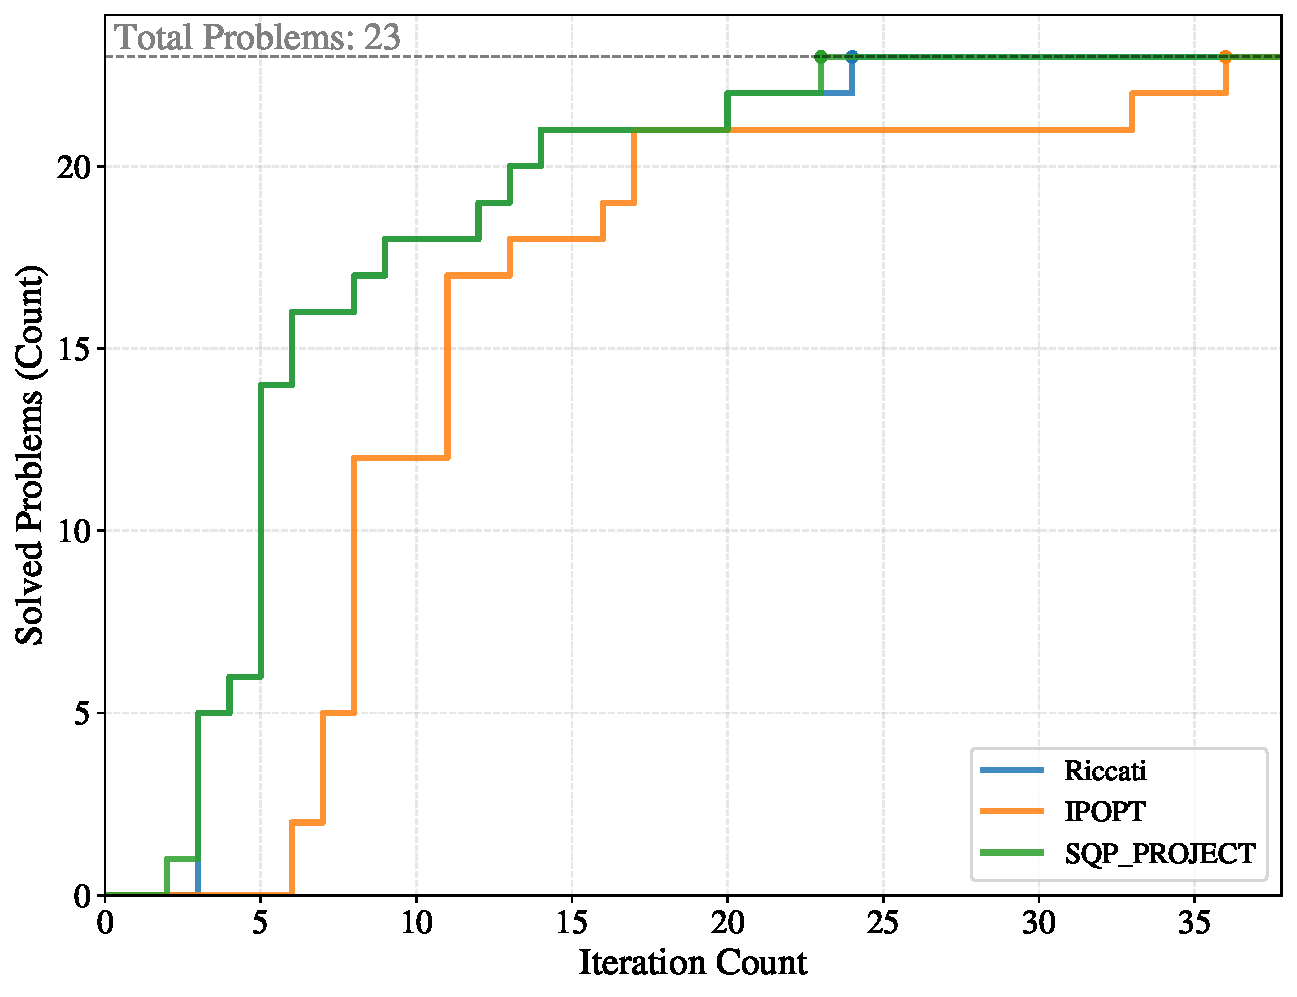
\includegraphics[width=0.65\textwidth]{results/iter_mehrotra_pos.pdf}
        \caption{Iteration results of the prototype solver on convex QPs}
    \end{figure}
\end{frame}

\begin{frame}
    \frametitle{Heuritic modification: Mehrotra predictor-corrector to Mehrotra probing}
    According to the paper \cite{nocedalAdaptiveBarrierUpdate2009a} from Nocedal et al.
    \vspace{0.2cm}

    "the direct extension of Mehrotra's predictor-corrector method to nonlinear programming does not result in a robust method."
    \vspace{0.2cm}

    They implemented the '\textbf{conditional Mehrotra predictor-corrector}' as heuristic to retain the performance in nonlinear programming, which is implemented in HPIPM as well as in the prototype.
    \vspace{0.2cm}

    Besides, they also described the mehtod that uses the heuristic for calculating the centering parameter $\sigma$ in Mehrotra's method but not using the corrector step, as '\textbf{Mehrotra probing}'.
    \vspace{0.2cm}

    I tried the Mehrotra probing method in the prototype solver, which proved to be less efficient in convex QPs but more robust in the nonconvex QPs.

\end{frame}

\begin{frame}
    \frametitle{Results II: Mehrotra Probing on convex QPs}
    \begin{figure}[H]
        \centering
        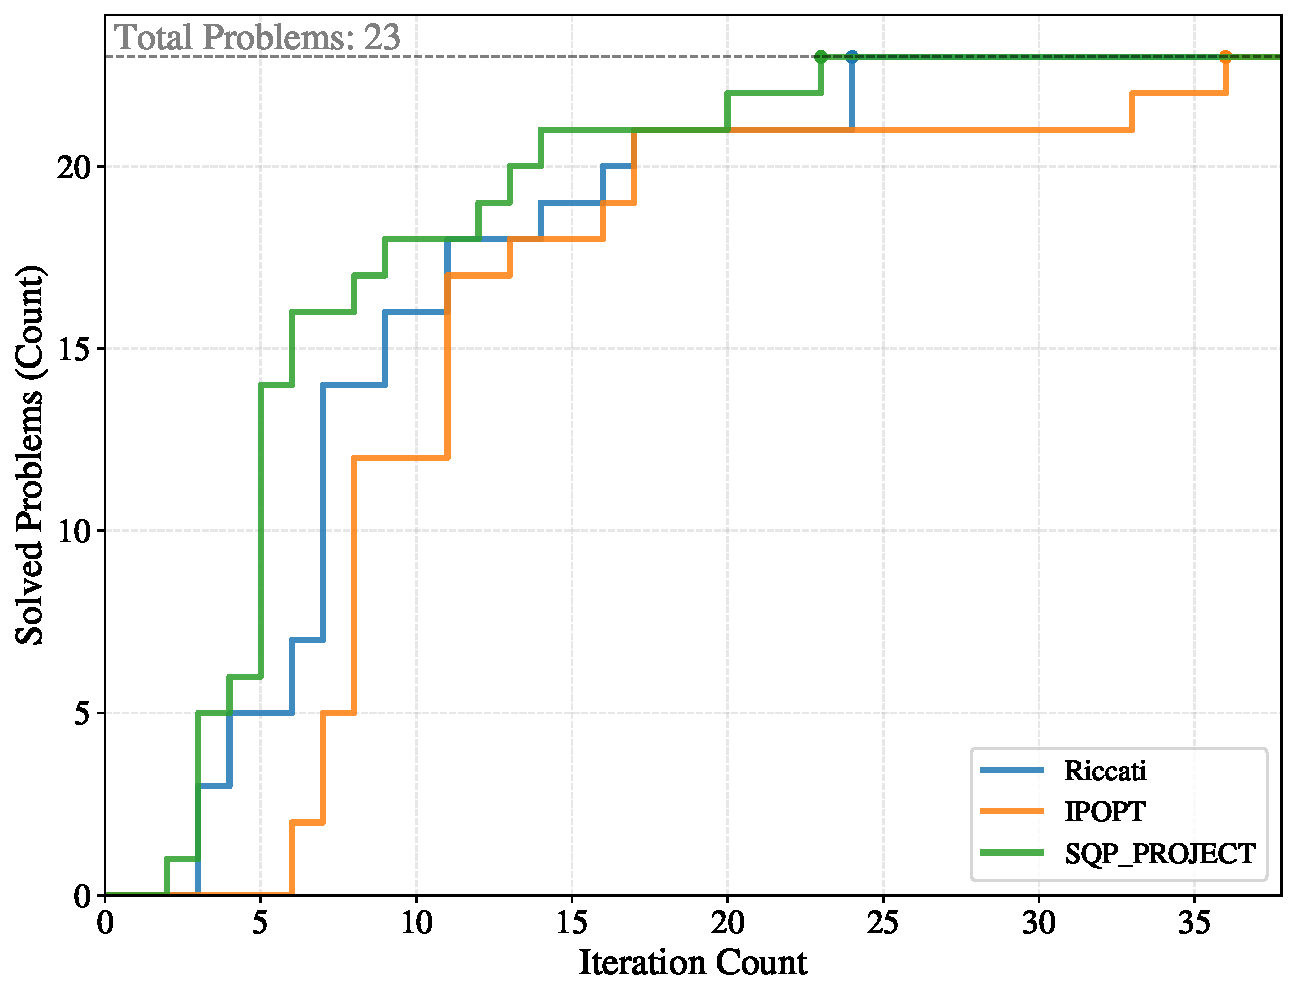
\includegraphics[width=0.65\textwidth]{results/iter_probing_pos.pdf}
        \caption{Iteration results of Mehrotras on convex QPs}
    \end{figure}
\end{frame}


\begin{frame}
    \frametitle{Results II: Mehrotra predictor-corrector on nonconvex QPs}
    \begin{figure}[H]
        \centering
        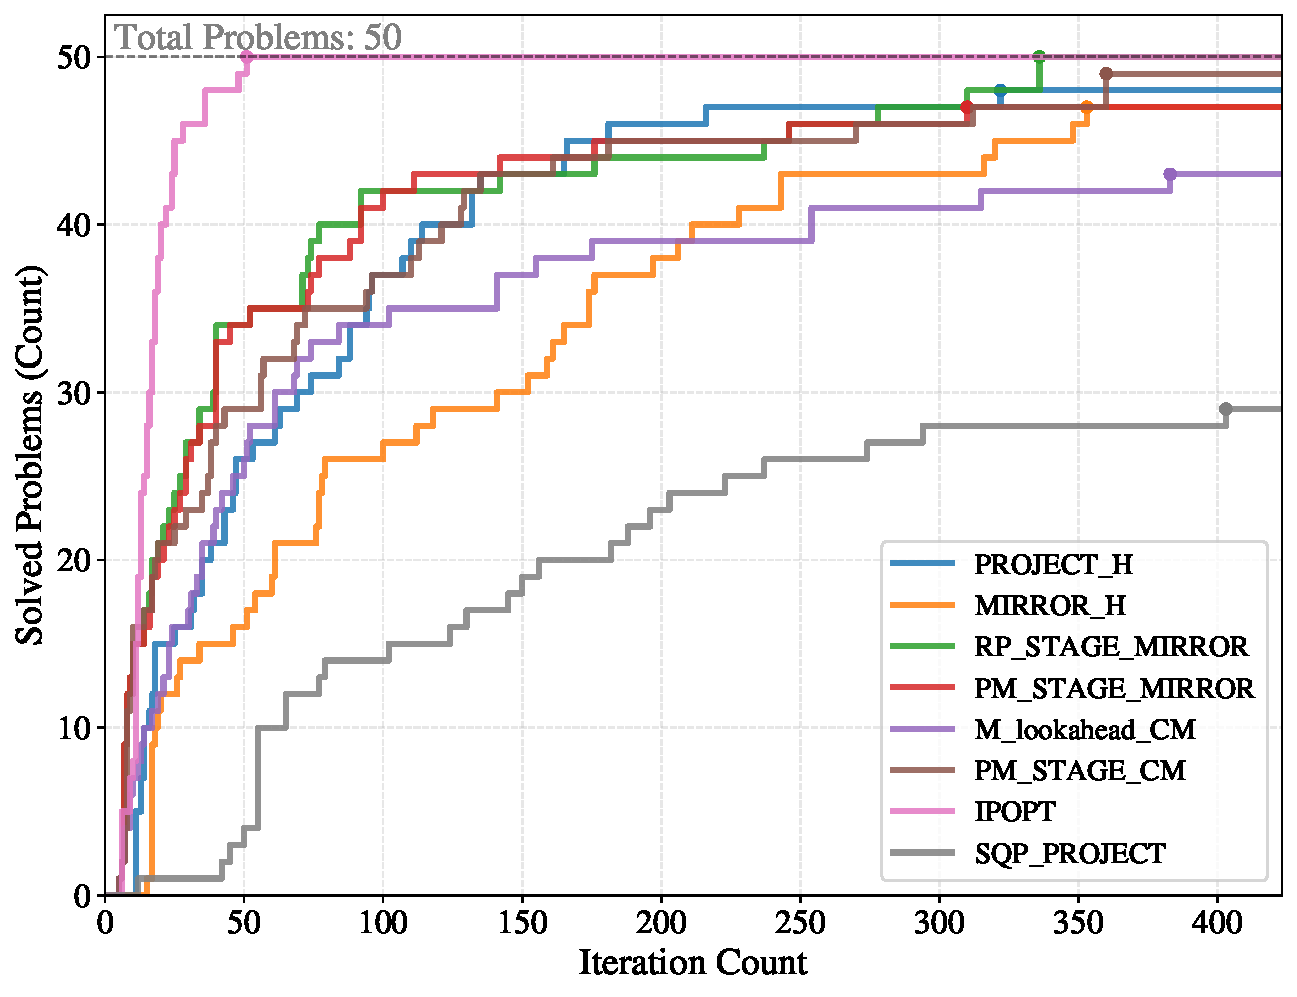
\includegraphics[width=0.65\textwidth]{results/iter_mehrotra_inde.pdf}
        \caption{Iteration results of Mehrotra predictor-corrector on nonconvex QPs}
    \end{figure}
\end{frame}

\begin{frame}
    \frametitle{Results II: Mehrotra probing on nonconvex QPs}
    \begin{figure}[H]
        \centering
        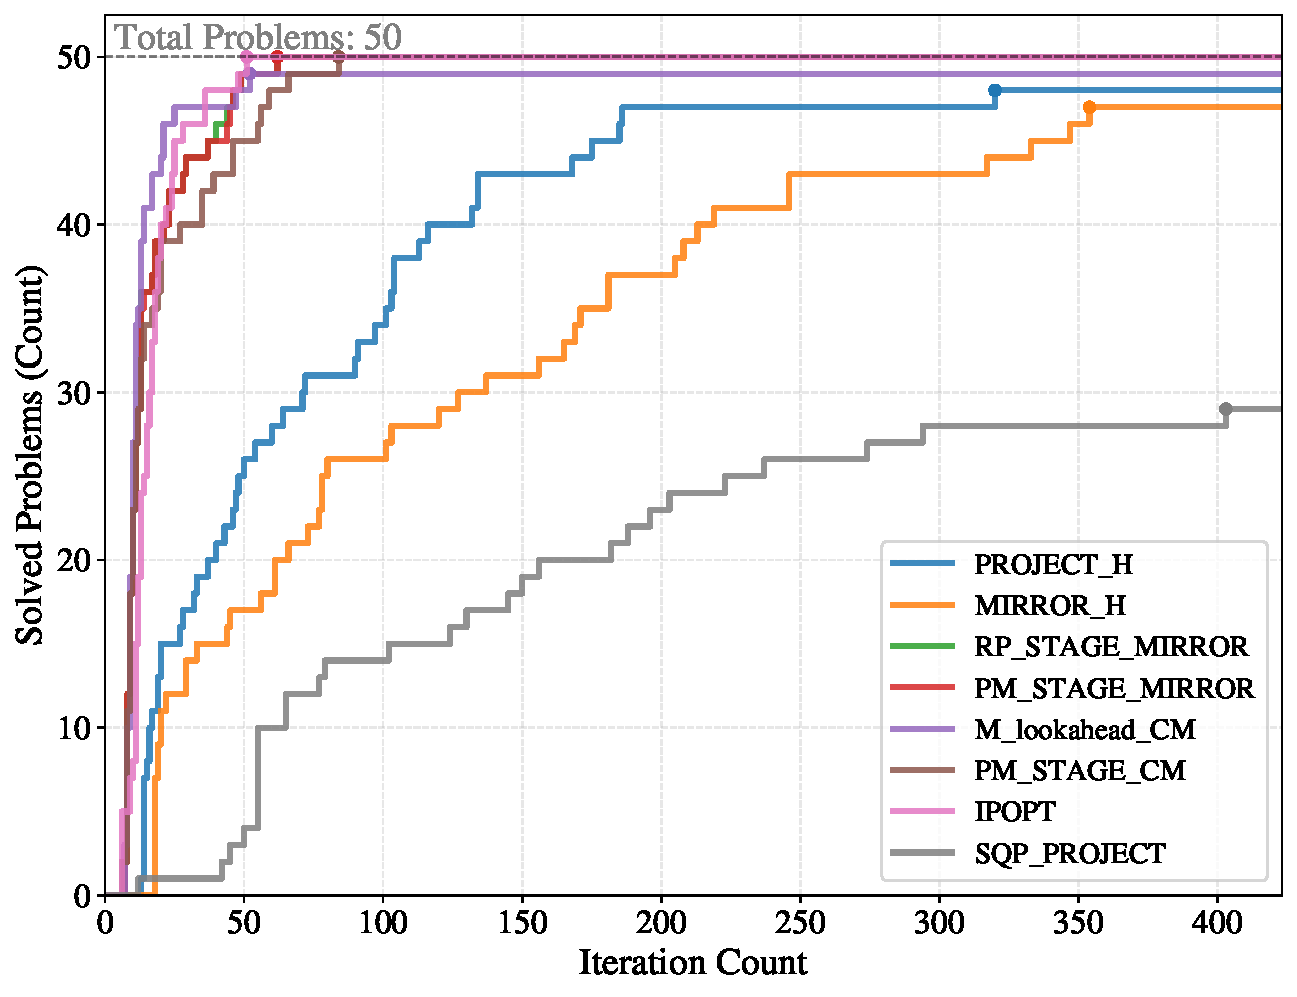
\includegraphics[width=0.65\textwidth]{results/iter_probing_inde.pdf}
        \caption{Iteration results of Mehrotra probing on nonconvex QPs}
    \end{figure}
\end{frame}

\begin{frame}
    \frametitle{Issue on the converged KKT point}
    \begin{figure}[H]
        \centering
        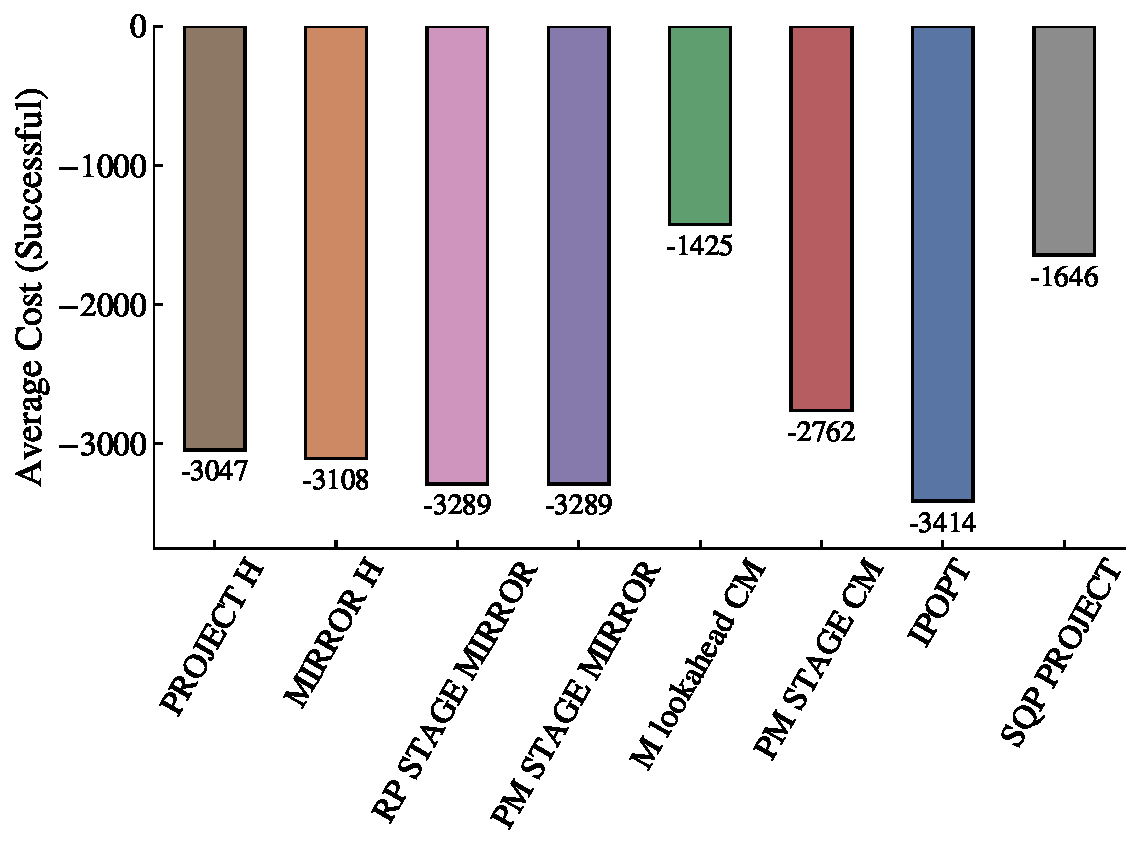
\includegraphics[width=0.65\textwidth]{results/cost_probing_inde.pdf}
        \caption{Average cost of Mehrotra probing on nonconvex QPs}
    \end{figure}
\end{frame}

\begin{frame}
    \frametitle{Theoretical aspect: Local quadratic convergence rate}
    According to the paper \cite{absilNewtonKKTInteriorpointMethods2007} from Absil et al.,
    we can prove the local quadratic convergence of the regularized interior point method if:
    \begin{itemize}
        \item The regularized Hessian is identical to the original Hessian of Newton's method when it is close to the solution.
        \item A full step length in primal and dual variables is taken when it is close to the solution.
    \end{itemize}
    \vspace{0.2cm}
    This is encouraging for giving a try on the proof of local quadratic convergence for the current algorithm, knowing:
    \begin{itemize}
        \item We only regularize reduced Hessian when Choleksy factorization fails during the Riccati recursion.
        \item The heuristic FTB in prototype usually ensures the full step length when it is close to the solution in practice.
        \begin{align*}
            \alpha_{p/d} &= 
            \begin{cases}
                \alpha_{\text{p/d}} \cdot \left( (1.0 - \alpha_{\text{p/d}}) \cdot 0.99 + \alpha_{\text{p/d}} \cdot 0.9999999 \right), & \text{if } \alpha_{\text{p/d}} < 1.0 \\
                1.0, & \text{if } \alpha_{\text{p/d}} \ge 1.0
            \end{cases}
        \end{align*}
    \end{itemize}
    Check the draft proof for details.
\end{frame}

\begin{frame}
    \frametitle{Globalization aspect: Funnel line search}
    According to \cite{kiesslingUnifiedFunnelRestoration2025} from David et al., three types of globalization strategies are usually discussed in the literature:
    \begin{itemize}
        \item Merit function
        \item Filter
        \item Funnel
    \end{itemize}
    And two types of globalization mechanisms are usually discussed:
    \begin{itemize}
        \item Line search
        \item Trust region
    \end{itemize}
    After some trials, the funnel line search is chosen and implemented in the prototype solver.
    \vspace{0.2cm}

    Unfortunately, to the best of my current knowledge, the proof of global convergence for the funnel line search is not provided by any literature yet.
\end{frame}

\begin{frame}
    \frametitle{Results III: Funnel line search on nonconvex QPs}
    \begin{figure}[H]
        \centering
        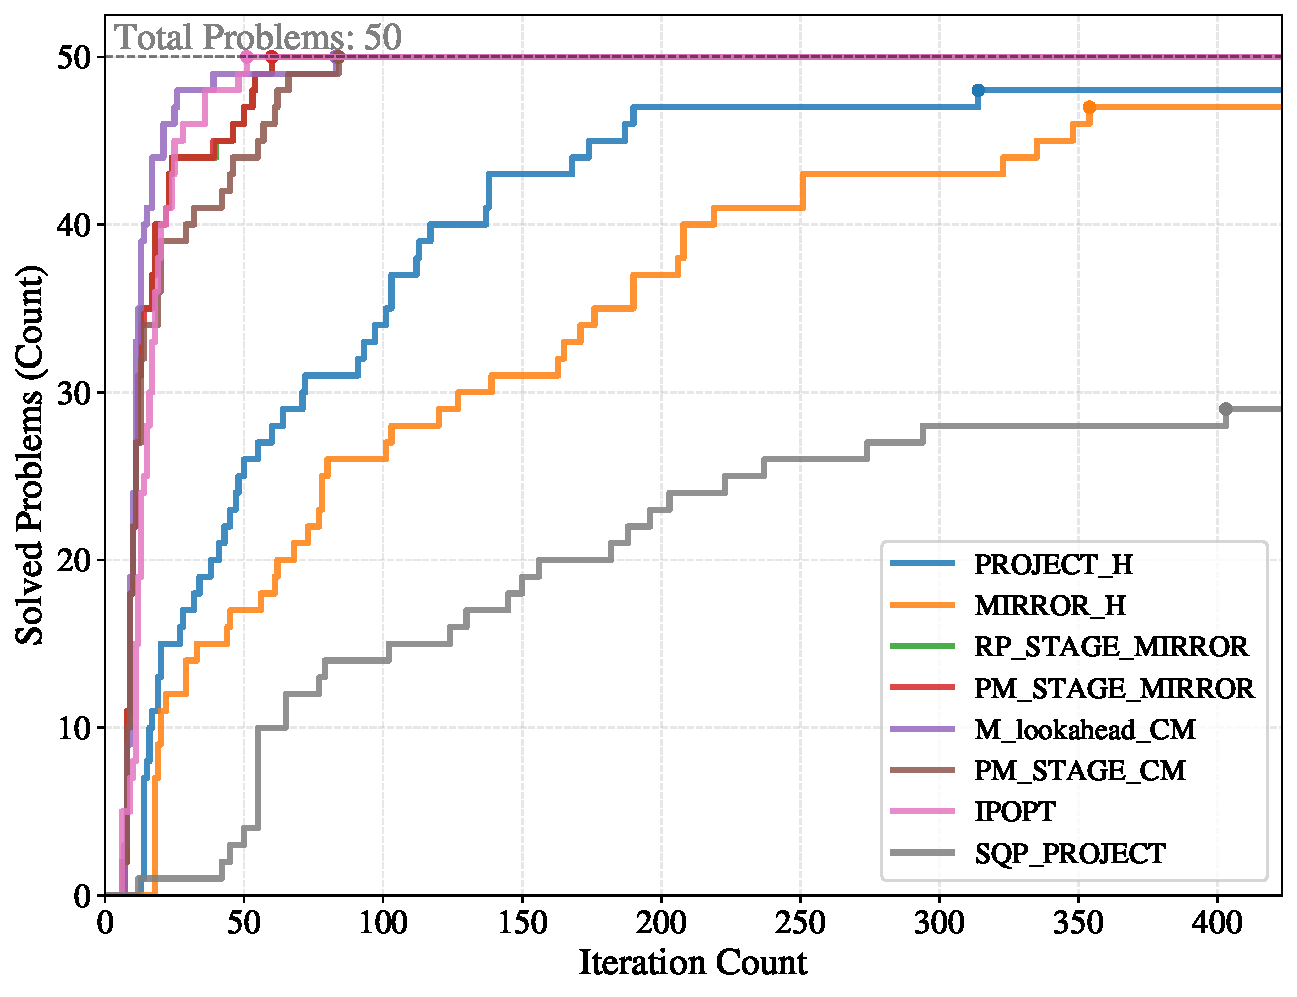
\includegraphics[width=0.65\textwidth]{results/iter_funnel_inde.pdf}
        \caption{Iteration results of funnel line search on nonconvex QPs}
    \end{figure}
\end{frame}


\begin{frame}
    \frametitle{Issue on the converged KKT point}
    \begin{figure}[H]
        \centering
        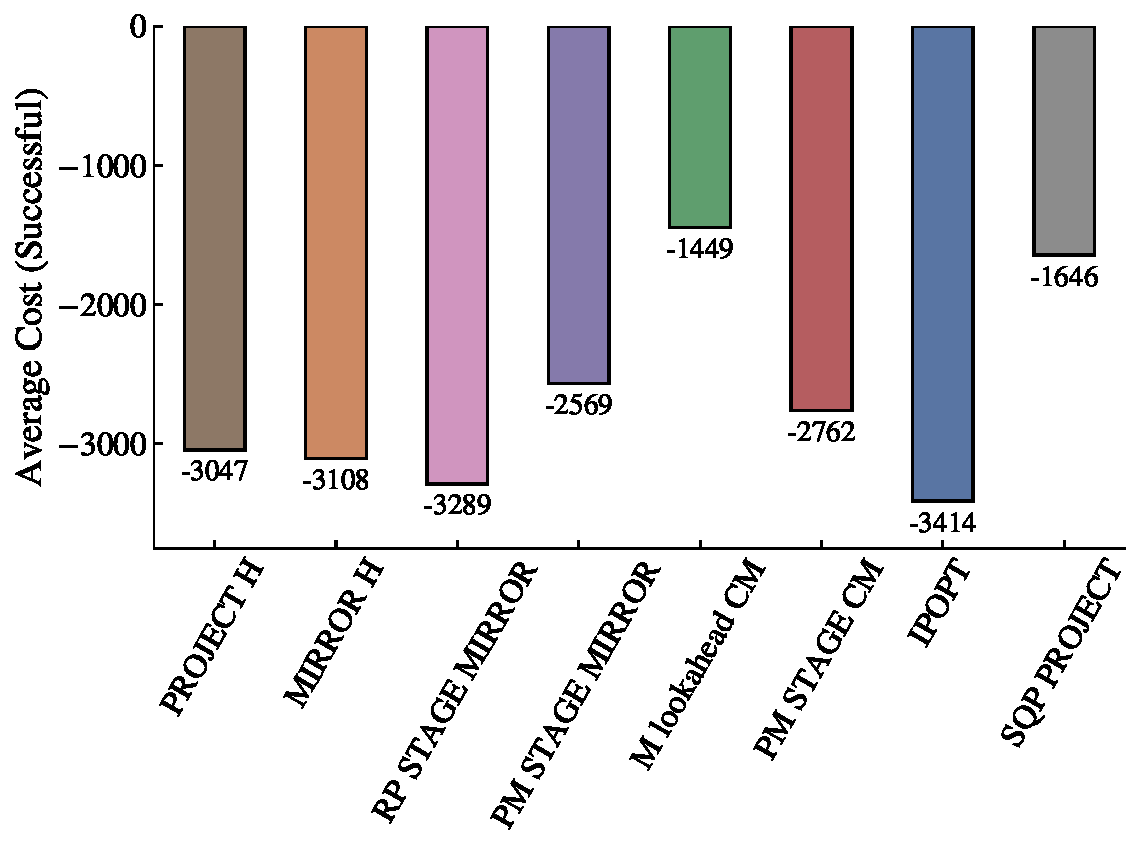
\includegraphics[width=0.65\textwidth]{results/cost_funnel_inde.pdf}
        \caption{Average cost of funnel line search on nonconvex QPs}
    \end{figure}
\end{frame}

\begin{frame}
    \frametitle{Some thoughts on next steps}
    Several things to ponder a bit:
    \begin{itemize}
        \item Engineering side:
        \begin{itemize}
            \item More test cases needed, maybe slack is needed for prototype.
            \item Performance in SQP: something next step
        \end{itemize}
        \item Theoretical side:
        \begin{itemize}
            \item Stage regularization:
            \begin{itemize}
            \item Bounds on Frobenius norm?
            \item Bounds on stage/full condition number?
            \end{itemize} 
            \item Local convergence proof: on the way, but quadratic convergence is very likely to be proved
            \item Global convergence proof: open question, but it could be something possible.
            \item Local minimizer quality: how to escape saddle points?
            \begin{itemize}
            \item Different regularization strategy?
            \item Better step size control strategy?
            \end{itemize}
        \end{itemize}
    \end{itemize}
\end{frame}


\bibliographystyle{IEEEtran}
\bibliography{references}

\end{document}
